\begin{filecontents*}{ie_refs.bib}
@article{zaratiana2023gliner,
  author  = {Urchade Zaratiana and Nadi Tomeh and Pierre Holat and Thierry Charnois},
  title   = {GLiNER: Generalist Model for Named Entity Recognition using Bidirectional Transformer},
  journal = {arXiv preprint arXiv:2311.08526},
  year    = {2023}
}
\end{filecontents*}

\documentclass[UTF8,a4paper,12pt]{ctexart}

\usepackage[a4paper,margin=2.2cm]{geometry}
\usepackage{amsmath,amssymb,bm}
\usepackage{booktabs}
\usepackage{array}
\usepackage{float}
\usepackage{caption}
\usepackage{hyperref}
\usepackage{xcolor}
\usepackage{listings}
\usepackage[ruled,vlined,linesnumbered]{algorithm2e}
\usepackage{tikz}
\usepackage{pgfplots}
\usetikzlibrary{arrows.meta,positioning,shapes.geometric,fit}
\pgfplotsset{compat=1.18}

\hypersetup{
  colorlinks=true,
  linkcolor=blue!45!black,
  citecolor=blue!45!black,
  urlcolor=blue!45!black
}

\definecolor{IEBlue}{RGB}{52,95,145}
\definecolor{IEGray}{RGB}{92,98,106}
\definecolor{IELight}{RGB}{239,243,247}

\lstset{
  basicstyle=\ttfamily\small,
  frame=single,
  breaklines=true,
  columns=fullflexible,
  backgroundcolor=\color{IELight},
  rulecolor=\color{black!15}
}

\SetKwInput{KwIn}{输入}
\SetKwInput{KwOut}{输出}
\SetKw{KwRet}{return}
\DontPrintSemicolon
\SetAlFnt{\small}
\renewcommand{\algorithmcfname}{算法}

\title{信息抽取实验报告\\规则系统与 GLiNER 联合抽取技能结构化信息}
\author{acknowledge 项目实验记录}
\date{\today}

\begin{document}
\maketitle

\begin{abstract}
这次实验做的是一个偏工程型的信息抽取系统：从 skills.sh 的技能描述里抽出平台、技术栈、动作类型、目标领域、输出格式和量化指标六类信息。系统没有直接押宝在一个模型上，而是拆成三层：baseline 做精确关键字匹配，enhanced-regex 在此基础上补 action alias、受控词表归一化和 fallback，enhanced-gliner 再把 GLiNER 作为前置候选生成器接进来。

按当前工作区里能复现的结果，\texttt{ground\_truth.json} 上的整体 F1 从 baseline 的 37.66\% 提到 enhanced-regex 的 60.36\%；当前 enhanced 输出对应的 GLiNER 版本 F1 为 59.78\%。也就是说，这批标注样本里真正把分数拉起来的还是规则增强层，GLiNER 没有继续抬高总分，反而在 \texttt{output\_formats} 上带来一点精度损失。不过把范围放回全量 1000 条数据，GLiNER 依然留下了 1624 条 \texttt{gliner\_direct} 和 582 条 \texttt{gliner\_normalized} 证据，说明它并不是完全没用，而是卡在词表和阈值这一层。
\end{abstract}

\section{引言}
这个子系统要解决的问题可以写得很具体：给一条技能描述，自动整理出它服务哪个平台、用什么技术、做什么动作、面向什么场景、最后产出什么格式。检索系统拿到这样的结构化结果后，界面展示和后续统计都会轻松很多，后面如果接问答或推荐，也不用每次都从长文本里硬抠关键词。

数据还是同一批 1000 条 skills.sh 记录。字段除了 \texttt{skill\_name}、\texttt{description}、\texttt{category} 这些主键，还包含外置的 \texttt{SKILL.md} 文本路径。当前快照里 917 条能读到外置技能文档，83 条缺 \texttt{SKILL.md}，203 条缺简介。文本语言整体偏英文，标题和描述同时含 CJK 的记录非常少，所以抽取系统里专门加了一个 \texttt{english\_only\_bias} 开关，避免 GLiNER 在非英文文本上乱猜。

这次实验最关心三件事：第一，baseline 和 enhanced-regex 到底各修掉了哪些问题；第二，GLiNER 接进来以后，收益是不是落在评测集能测到的地方；第三，如果模型命中了 span 但最后还是没被系统接住，瓶颈究竟出在词表、阈值还是后处理。

\section{数据获取与预处理}
\subsection{抓取与 checkpoint 流程}
IE 系统用的数据不是另外造的，而是直接吃 \texttt{paqu.py} 写下来的共享数据集。抓取流程和 IR 报告一致，这里仍然给出一张图，方便后面解释为什么有的文本来自 \texttt{description}，有的来自外置 \texttt{SKILL.md}。

\begin{figure}[H]
\centering
\begin{tikzpicture}[
  node distance=8mm and 10mm,
  box/.style={rounded corners, draw=IEBlue!65, fill=IELight, minimum width=27mm, minimum height=8mm, align=center},
  line/.style={-{Latex[length=2.5mm]}, thick, draw=IEGray}
]
\node[box] (home) {滚动首页\\收集 URL};
\node[box, right=of home] (detail) {拉取详情页 HTML};
\node[box, right=of detail] (parse) {解析字段\\与 SSR 片段};
\node[box, below=of parse] (skillmd) {补抓完整\\\texttt{SKILL.md}};
\node[box, left=of skillmd] (norm) {字段规范化\\数值清洗 / URL 规整};
\node[box, left=of norm] (save) {写入主数据\\外置文本文件};
\node[box, below=of detail] (ckpt) {checkpoint\\失败重试 / 断点续跑};

\draw[line] (home) -- (detail);
\draw[line] (detail) -- (parse);
\draw[line] (parse) -- (skillmd);
\draw[line] (skillmd) -- (norm);
\draw[line] (norm) -- (save);
\draw[line] (detail) -- (ckpt);
\draw[line] (parse) -- (ckpt);
\draw[line] (save) |- (ckpt);
\draw[line] (ckpt.west) -| ([xshift=-8mm]home.west) |- (home.south);
\end{tikzpicture}
\caption{IE 使用的数据准备链路：抓取和清洗在共享爬虫阶段完成，抽取模块拿到的是已经规范化过的主字段和外置 \texttt{SKILL.md} 文本。}
\label{fig:ie-paqu-flow}
\end{figure}

\subsection{字段与文本来源}
抽取阶段真正关心的是表 \ref{tab:ie-fields} 这些字段。它们分别用于构造输入文本、辅助规则匹配和记录结果来源。

\begin{table}[H]
\centering
\caption{IE 子系统直接使用的主要字段}
\label{tab:ie-fields}
\begin{tabular}{p{3.3cm}p{8.2cm}r}
\toprule
字段名 & 作用 & 非空条数 \\
\midrule
\texttt{skill\_name} & 事件标题，构造 \texttt{full\_text} 与 \texttt{gliner\_text} & 1000 \\
\texttt{description} & 短摘要，GLiNER 的主要上下文之一 & 797 \\
\texttt{category} & 类别先验，常和领域词一起进入输入文本 & 1000 \\
\texttt{skill\_md\_text\_path} & 长文本主来源，覆盖率最高 & 917 \\
\texttt{skill\_md\_raw\_text\_path} & 保留原始换行，便于正则抽取 metrics & 917 \\
\texttt{detail\_url} & 回看样本和误差分析时的定位键 & 1000 \\
\bottomrule
\end{tabular}
\end{table}

代码里读文本的优先级是
\[
\texttt{external\_skill\_text} > \texttt{skill\_md\_raw\_text} > \texttt{skill\_md} > \texttt{description}.
\]
这一步很关键。像 \texttt{maishou} 这种技能，如果只看简介，平台名单根本不完整；而像 \texttt{domain-authority-auditor} 这种长规则说明文档，如果直接把整段都丢给 baseline，又会触发一堆过宽的动词和领域词。

\subsection{预处理：文本包与语言偏置}
抽取前，系统会为每个文档构造三个视图：
\begin{itemize}
  \item \texttt{full\_text}：\texttt{skill\_name + category + extraction\_text}，供完整规则匹配使用；
  \item \texttt{gliner\_text}：压缩过的聚焦文本，避免超长输入把 GLiNER 拖慢；
  \item \texttt{fallback\_text}：GLiNER 失败或跳过后回退使用的文本。
\end{itemize}

语言偏置判断写得很直白。设文本里的 ASCII 字母数为 $n_{\text{ascii}}$，CJK 字符数为 $n_{\text{cjk}}$，则
\begin{equation}
\label{eq:english-bias}
\texttt{english\_dominant}(x)=
\begin{cases}
1, & n_{\text{cjk}}=0,\\
1, & n_{\text{ascii}}\ge 1.5\,n_{\text{cjk}},\\
0, & \text{otherwise}.
\end{cases}
\end{equation}

当 \texttt{english\_only\_bias=true} 且式 \eqref{eq:english-bias} 判成 0 时，GLiNER 直接跳过，系统退回规则路径。这个判断不花哨，但和当前数据的语言分布是对得上的。

\section{核心算法}
\subsection{三阶段结构}
这套 IE 系统不是单一模型，而是三层递进关系。图 \ref{fig:ie-variant-flow} 画出了它们的区别。

\begin{figure}[H]
\centering
\begin{tikzpicture}[
  node distance=8mm and 10mm,
  box/.style={rounded corners, draw=IEBlue!70, fill=IELight, minimum width=30mm, minimum height=8mm, align=center},
  decision/.style={diamond, draw=IEBlue!70, fill=white, aspect=2, inner sep=1pt, align=center},
  line/.style={-{Latex[length=2.5mm]}, thick, draw=IEGray}
]
\node[box] (input) {输入文本包\\\texttt{full\_text / gliner\_text}};
\node[box, right=of input] (base) {Stage 1\\baseline\\精确关键字 + metrics 正则};
\node[box, right=of base] (regex) {Stage 2\\enhanced-regex\\词表归一化 + alias + fallback};
\node[decision, below=of regex] (lang) {英文主导?};
\node[box, right=of regex] (gliner) {Stage 3\\enhanced-gliner\\GLiNER 候选 + 阈值过滤};
\node[box, below=of gliner] (merge) {归一化 / fallback / 合并证据};
\node[box, left=of merge] (out) {结构化结果\\+ evidence};

\draw[line] (input) -- (base);
\draw[line] (base) -- (regex);
\draw[line] (regex) -- (gliner);
\draw[line] (regex) -- (lang);
\draw[line] (lang.east) -| node[pos=0.25,above right] {\small 是} (gliner.south);
\draw[line] (lang.west) -| node[pos=0.25,above left] {\small 否} (merge.west);
\draw[line] (gliner) -- (merge);
\draw[line] (merge) -- (out);
\end{tikzpicture}
\caption{IE 三阶段结构：baseline 先给出纯规则底线，enhanced-regex 负责把 alias、归一化和 fallback 接起来，GLiNER 则只在英文主导文本上提供额外候选。}
\label{fig:ie-variant-flow}
\end{figure}

实际跑下来，第二层提升最大，第三层并没有稳定继续加分。这一点后面看结果时会非常明显。

\subsection{baseline：精确关键字与 metrics 正则}
baseline 对五个枚举字段都走 \verb|\bkeyword\b| 形式的正则精确匹配，配置项来自 \texttt{ie\_config.json}。这样做的好处是行为很可审计，坏处也同样明显：词表一旦偏窄，FN 会很多；词表一旦偏宽，FP 也会很多。

\texttt{metrics} 字段单独处理，不靠关键字表，而是靠四组模式去抓“数字 + 单位”：
\begin{table}[H]
\centering
\caption{metrics 字段使用的主要正则模式与示例}
\label{tab:metric-regex}
\begin{tabular}{p{6.0cm}p{5.8cm}}
\toprule
模式 & 典型命中示例 \\
\midrule
\texttt{(\textbackslash d+)[-\textbackslash s]*(signal|criteria|item|...)} & \texttt{5-signal}, \texttt{12-criteria} \\
\texttt{(?:across|over|with|covering|spanning)\textbackslash s+(\textbackslash d+)\textbackslash s+...} & \texttt{across 8 dimensions} \\
\texttt{(\textbackslash d+)\textbackslash s*[---]\textbackslash s*(\textbackslash d+)\textbackslash s*(?:scale|score|range|rating)} & \texttt{1-10 scale} \\
\texttt{supports five modules} 这类英文数字模式 & \texttt{supports five modules} \\
\bottomrule
\end{tabular}
\end{table}

这部分设计得挺实用，因为 metrics 往往混在说明文字里，硬列词表意义不大。

\subsection{enhanced-regex：alias 扩展与受控词表归一化}
第二层增强主要做两件事。第一件是 action alias 扩展，例如 \texttt{analysis}、\texttt{analytics}、\texttt{analyzer} 都归到 \texttt{analyze}，\texttt{writer}、\texttt{writing}、\texttt{drafting} 都归到 \texttt{create}。第二件是受控词表归一化，顺序是：
\begin{equation}
\label{eq:norm-chain}
\text{exact} \rightarrow \text{folded} \rightarrow \text{alias} \rightarrow \text{fuzzy} \rightarrow \text{unknown}.
\end{equation}

\texttt{folded} 匹配会把大小写和符号折叠，例如 \texttt{node.js} 和 \texttt{nodejs} 归到同一项；\texttt{alias} 匹配再处理 \texttt{github.com} $\rightarrow$ \texttt{github}、\texttt{jd} $\rightarrow$ \texttt{jd.com} 这种别名；最后还有一个编辑距离不超过 2 的模糊匹配，用来救一下明显的轻微拼写变体。

这层增强是这次实验里真正的主力。拿 \texttt{maishou} 来说，baseline 只能抓到 \texttt{1688}，enhanced-regex 则能把 \texttt{taobao}、\texttt{tmall}、\texttt{jd.com}、\texttt{pinduoduo}、\texttt{vip.com} 一次性补齐。

\subsection{GLiNER 集成与阈值门控}
第三层把 GLiNER 接进来做候选实体提取\cite{zaratiana2023gliner}。它在系统里的位置不是“直接产出最终答案”，而是“先提 span，再让规则层决定要不要收下”。整条链路见图 \ref{fig:gliner-flow}。

\begin{figure}[H]
\centering
\begin{tikzpicture}[
  node distance=8mm and 10mm,
  box/.style={rounded corners, draw=IEBlue!70, fill=IELight, minimum width=30mm, minimum height=8mm, align=center},
  decision/.style={diamond, draw=IEBlue!70, fill=white, aspect=2, inner sep=1pt, align=center},
  line/.style={-{Latex[length=2.5mm]}, thick, draw=IEGray}
]
\node[box] (bundle) {构造 \texttt{gliner\_text}\\与语言标签};
\node[decision, right=of bundle] (eligible) {可走 GLiNER?};
\node[box, right=of eligible] (predict) {GLiNER 推理\\输出 span, label, score};
\node[box, below=of predict] (project) {标签映射到字段\\按阈值过滤};
\node[box, left=of project] (normalize) {词表归一化\\exact / alias / fuzzy};
\node[box, below=of normalize] (fallback) {字段 fallback\\关键字补抽};
\node[box, right=of fallback] (result) {合并 values\\保留 evidence};

\draw[line] (bundle) -- (eligible);
\draw[line] (eligible) -- node[above] {\small 是} (predict);
\draw[line] (eligible.south) |- node[pos=0.2,left] {\small 否} (fallback.west);
\draw[line] (predict) -- (project);
\draw[line] (project) -- (normalize);
\draw[line] (normalize) -- (fallback);
\draw[line] (fallback) -- (result);
\end{tikzpicture}
\caption{GLiNER 在系统里的实际位置：模型只负责给候选 span 和分数，真正决定保留什么字段的仍然是阈值、受控词表和 fallback 规则。}
\label{fig:gliner-flow}
\end{figure}

字段阈值是手工设的，表 \ref{tab:thresholds} 给出当前配置。

\begin{table}[H]
\centering
\caption{GLiNER 各字段的置信度阈值}
\label{tab:thresholds}
\begin{tabular}{lc}
\toprule
字段 & 阈值 \\
\midrule
\texttt{platforms} & 0.4 \\
\texttt{languages} & 0.3 \\
\texttt{action\_types} & 0.5 \\
\texttt{target\_domains} & 0.5 \\
\texttt{output\_formats} & 0.3 \\
\texttt{metrics} & 0.6 \\
\bottomrule
\end{tabular}
\end{table}

形式上可以写成
\begin{equation}
\label{eq:threshold}
\text{accept}(x,f)=
\begin{cases}
1, & \operatorname{score}(x,f)\ge \tau_f,\\
0, & \operatorname{score}(x,f)< \tau_f.
\end{cases}
\end{equation}

如果一个 span 过了阈值，但归一化后找不到合法词表项，系统不会静默吞掉，而是把它记成 \texttt{gliner\_unknown}。这一点对误差分析很有用。

\subsection{增强版抽取流程伪代码}
算法 \ref{alg:ie-enhanced} 把第三层增强流程压缩成伪代码。它和真实实现最接近的地方，是把“模型命中”和“规则回退”放在了同一条流水线上，而不是两个独立系统。

\begin{algorithm}[H]
\caption{enhanced 抽取主流程}
\label{alg:ie-enhanced}
\KwIn{文档 $d$}
\KwOut{抽取结果 $E$ 与证据映射 $V$}

$B \leftarrow \textsc{BuildTextBundle}(d)$\;
\If{$\texttt{variant}=\texttt{baseline}$}{
  \KwRet \textsc{ExactKeywordExtract}$(B.\texttt{full\_text})$\;
}

\If{$B.\texttt{gliner\_eligible}$ 且模型可用}{
  $P \leftarrow \textsc{PredictGLiNER}(B.\texttt{gliner\_text})$\;
  $H \leftarrow \textsc{ProjectByField}(P,\tau_f)$\;
}
\Else{
  $H \leftarrow \varnothing$\;
}

\ForEach{枚举字段 $f$}{
  \If{$H[f]$ 有可归一化命中}{
    $E[f] \leftarrow \textsc{NormalizeToVocab}(H[f])$\;
    $E[f] \leftarrow \textsc{MergeFallback}(E[f],B.\texttt{fallback\_text})$\;
  }
  \Else{
    $E[f] \leftarrow \textsc{FallbackExtract}(f,B.\texttt{fallback\_text})$\;
  }
}
$E[\texttt{metrics}] \leftarrow \textsc{MetricRegex}(B.\texttt{full\_text},H[\texttt{metrics}])$\;
\KwRet $(E,V)$\;
\end{algorithm}

\section{实验设计与过程}
\subsection{实验环境}
实验仍然在 Windows 10（\texttt{10.0.26100}）上完成，conda 环境是 \texttt{yolov82}，Python 版本 3.11.5。GLiNER 按配置跑在 CPU 上，模型缓存目录位于 \texttt{ie\_system/runtime/gliner\_cache/}。第一次加载模型时冷启动很明显，在本机上频繁全量重跑并不轻松，这也是我后面尽量复用现有输出文件的原因。

\subsection{标注集与评测办法}
自动评测集是 \texttt{ie\_system/eval/ground\_truth.json}，共 10 条 skill，每条标注五个枚举字段：\texttt{platforms}、\texttt{languages}、\texttt{action\_types}、\texttt{target\_domains}、\texttt{output\_formats}。虽然系统内部也抽 \texttt{metrics}，但它的值是 \texttt{\{value, unit\}} 字典列表，直接做集合交并不合适，所以自动评测把它排除在外。

Precision、Recall、F1 的定义仍然是集合式写法：
\begin{align}
\label{eq:prf}
P &= \frac{|Y \cap \hat{Y}|}{|\hat{Y}|},\\
R &= \frac{|Y \cap \hat{Y}|}{|Y|},\\
F1 &= \frac{2PR}{P+R},
\end{align}
其中 $Y$ 是人工标注集合，$\hat{Y}$ 是系统抽取集合。

这里有个实际问题必须记下来：当前数据快照里，标注集中的 \texttt{pdf-converter} 不在 \texttt{skills\_data.json} 里，所以自动评测最终只匹配到 9 条文档。这个坑不是算法问题，是数据版本没完全对齐。为了把三阶段表做完整，我保留了现有 runtime 结果，同时补跑了不启用 GLiNER 的 regex 阶段来对齐数值。

\subsection{运行命令}
\begin{lstlisting}[language=bash,caption={IE 子系统的主要运行命令}]
python ie_system/skills_ie_system.py extract --variant enhanced
python ie_system/skills_ie_system.py evaluate --variant enhanced --eval-set ground_truth.json
python ie_system/skills_ie_system.py compare --eval-set ground_truth.json
python ie_system/skills_ie_system.py report --variant enhanced
\end{lstlisting}

其中：
\begin{itemize}
  \item \texttt{comparison\_report.json} 更适合看 baseline 和 regex 增强层；
  \item \texttt{evaluation\_report.json} 与 \texttt{output/extraction\_results.json} 对应当前 enhanced 输出；
  \item \texttt{extraction\_report.json} 记录的是全量 1000 条文档的覆盖率和证据来源。
\end{itemize}

\section{实验结果与对比分析}
\subsection{三阶段总表}
表 \ref{tab:ie-overall} 给出三阶段的总结果。这里的 Stage 2 是我按当前代码补跑的 \texttt{enhanced-regex}；Stage 3 使用的是当前仓库里已经落盘的 enhanced 输出评测值。

\begin{table}[H]
\centering
\caption{IE 三阶段整体 P/R/F1 对比}
\label{tab:ie-overall}
\begin{tabular}{lccc}
\toprule
阶段 & Precision & Recall & F1 \\
\midrule
Stage 1: baseline & 0.3321 & 0.4348 & 0.3766 \\
Stage 2: enhanced-regex & \textbf{0.5971} & \textbf{0.6102} & \textbf{0.6036} \\
Stage 3: enhanced-gliner & 0.5860 & \textbf{0.6102} & 0.5978 \\
\bottomrule
\end{tabular}
\end{table}

这个结果不算“模型加进来就大获全胜”的故事。真正把 F1 从 37.66\% 拉到 60.36\% 的，是 alias 扩展、词表归一化和字段 fallback。GLiNER 在当前评测集上没有再把总分抬高，反而因为 Precision 略掉了一点，最终 F1 比 regex 低 0.58 个百分点。

\subsection{分字段 F1 对比}
图 \ref{fig:ie-field-f1} 把五个自动评测字段的 F1 拆开看。平台字段的提升最猛：baseline 只有 0.4118，到了 regex 阶段直接到 1.0000。GLiNER 阶段四个字段维持不变，只有 \texttt{output\_formats} 从 0.4375 掉到 0.4000。

\begin{figure}[H]
\centering
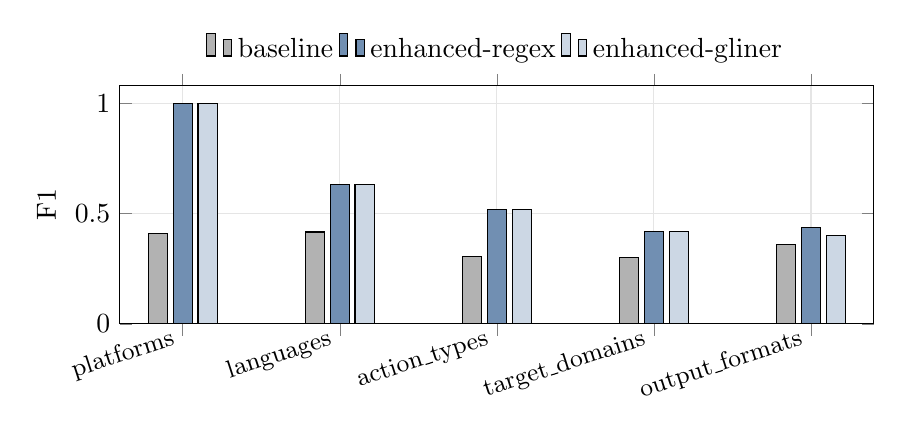
\begin{tikzpicture}
\begin{axis}[
  ybar,
  bar width=7pt,
  width=0.92\textwidth,
  height=0.38\textwidth,
  ymin=0, ymax=1.08,
  ylabel={F1},
  symbolic x coords={platforms,languages,action\_types,target\_domains,output\_formats},
  xtick=data,
  xticklabel style={font=\small, rotate=18, anchor=east},
  legend style={at={(0.5,1.05)}, anchor=south, legend columns=3, draw=none},
  grid=major,
  grid style={draw=black!10}
]
\addplot[fill=black!30] coordinates {
  (platforms,0.4118)
  (languages,0.4167)
  (action\_types,0.3076)
  (target\_domains,0.2991)
  (output\_formats,0.3617)
};
\addplot[fill=IEBlue!70] coordinates {
  (platforms,1.0000)
  (languages,0.6338)
  (action\_types,0.5185)
  (target\_domains,0.4208)
  (output\_formats,0.4375)
};
\addplot[fill=IEBlue!25] coordinates {
  (platforms,1.0000)
  (languages,0.6338)
  (action\_types,0.5185)
  (target\_domains,0.4208)
  (output\_formats,0.4000)
};
\legend{baseline, enhanced-regex, enhanced-gliner}
\end{axis}
\end{tikzpicture}
\caption{五个自动评测字段的 F1 柱状图：规则增强层把平台、动作和语言字段拉高了一大截；GLiNER 阶段在当前标注集上没有继续扩大优势，反而让 \texttt{output\_formats} 略有回落。}
\label{fig:ie-field-f1}
\end{figure}

这张图和表 \ref{tab:ie-overall} 放在一起看，结论就比较清楚了：当前评测集更奖励“可控的规则增强”，而不是“模型先猜一遍再交给规则兜底”。这不代表 GLiNER 没价值，只能说明现在的标注样本还没有把它的价值测出来。

\subsection{全量 1000 条覆盖率}
为了不只盯着 9 条可对齐样本，我又看了全量 \texttt{extraction\_report.json}。当前 enhanced 输出在 1000 条文档上的字段覆盖率是：
\begin{itemize}
  \item \texttt{platforms}: 24.5\%
  \item \texttt{languages}: 44.0\%
  \item \texttt{action\_types}: 87.2\%
  \item \texttt{target\_domains}: 92.7\%
  \item \texttt{output\_formats}: 47.2\%
  \item \texttt{metrics}: 13.7\%
\end{itemize}

证据来源分布也挺有意思。全局最多的是 \texttt{keyword\_fallback}（8362 条），其次是 \texttt{gliner\_unknown}（5062 条）、\texttt{alias\_fallback}（1900 条）、\texttt{gliner\_direct}（1624 条）和 \texttt{gliner\_normalized}（582 条）。这说明 GLiNER 其实命中过不少 span，但很多 span 最后停在了“模型看见了，词表收不下”这一步。

\subsection{误差分析}
这部分我只挑最典型的坑，不把所有 bad case 都平铺出来。

\paragraph{1. 关键字过宽带来的 FP}
\texttt{domain-authority-auditor} 在 baseline 下的 \texttt{action\_types} 特别典型。标注期望只有 \texttt{audit/detect/evaluate}，系统却能抽出 \texttt{build}、\texttt{compare}、\texttt{generate}、\texttt{report}、\texttt{review}、\texttt{validate} 一大串。问题不在正则写错，而在这类技能文档本来就像操作手册，动词太密了。只要看到词就收，Precision 一定扛不住。

\paragraph{2. 词表覆盖不够，FN 还是会留下}
\texttt{frontend-design} 的 \texttt{target\_domains} 期望里有 \texttt{ui}，系统长期抽不出来；\texttt{manim-composer} 的 \texttt{languages} 期望里有 \texttt{python}，系统只抓到 \texttt{manim}；\texttt{write-xiaohongshu} 的 \texttt{target\_domains} 期望是 \texttt{content/copywriting/social media}，结果当前输出还是偏到 \texttt{ai/frontend}。这些例子都说明词表还不够细，尤其是“领域词”和“技术词”之间有不少边界模糊的地方。

\paragraph{3. GLiNER 命中了，但归一化层没有接住}
全量输出里一共有 5062 条 \texttt{gliner\_unknown}，其中 \texttt{platforms} 2310 条、\texttt{languages} 1639 条、\texttt{output\_formats} 585 条、\texttt{action\_types} 512 条、\texttt{target\_domains} 16 条。样例里能看到不少很真实的卡点：
\begin{itemize}
  \item \texttt{geo-content-optimizer} 里出现 \texttt{ChatGPT}、\texttt{Claude}、\texttt{Perplexity}，模型看到了，但平台词表里没有；
  \item \texttt{schema-markup-generator} 里有 \texttt{Schema.org}，被打成 \texttt{platforms} 的 unknown；
  \item \texttt{actionbook} 里有 \texttt{CDP}、\texttt{Unix}，模型给了 \texttt{languages} 候选，但当前词表不认。
\end{itemize}

\paragraph{4. GLiNER 也会带来新的误判}
\texttt{manim-composer} 在当前 enhanced 输出里多了一个 \texttt{output\_formats=markdown}，而 regex 阶段是空值。还有 \texttt{frontend-design}，GLiNER 版本把 \texttt{output\_formats} 从 \texttt{html,json} 收缩到只有 \texttt{html}，虽然去掉了一个 FP，但也没把期望的 \texttt{css} 补回来。换句话说，模型不是纯增益项，它也会改变规则层本来已经形成的平衡。

\section{总结与展望}
这次 IE 实验最直接的结论是：规则层改得对不对，比模型是不是接进来更关键。baseline 的问题主要是“见词就收”，Precision 被拖得很低；regex+alias 一接上，平台、动作和语言字段马上好看很多。GLiNER 在当前标注集上没有继续抬高总分，但它留下了不少有价值的候选和 \texttt{unknown} 证据，这些信息对下一轮扩词表很有用。

系统现在的短板也很集中。标注集只有 10 条，而且其中 1 条缺失在当前数据快照里；GLiNER 只在英文主导文本上启用，中文和 mixed 文本基本还是靠规则；平台和语言词表偏窄，遇到 \texttt{ChatGPT}、\texttt{Claude}、\texttt{Perplexity}、\texttt{Schema.org} 这种新词就会掉进 \texttt{gliner\_unknown}；CPU 上的模型冷启动也比较慢，不适合频繁大批量重跑。

后面如果继续做，我会优先补三件事。第一，扩受控词表和别名，尤其把这次 \texttt{unknown} 里反复出现的实体收进去。第二，把 \texttt{metrics} 单独做一套更像样的评测，不再只停在“能抽出来几个”这个层面。第三，如果机器条件允许，直接换 GPU 跑 GLiNER，再看看阈值和英文偏置是不是还能放宽一点。

\bibliographystyle{gbt7714-numerical}
\bibliography{ie_refs}

\end{document}
